\documentclass[14pt,a4paper]{extarticle}

% Підтримка шрифтів та української мови (виключно Times New Roman, жодного італіка)
\usepackage{fontspec}
\usepackage{polyglossia}
\setdefaultlanguage{ukrainian}
\setmainfont{Times New Roman}

% Вимикаємо автопереноси
\hyphenpenalty=10000
\exhyphenpenalty=10000
\emergencystretch=3.5em
\sloppy

% Поля сторінки: ліве 30 мм, праве 15 мм, верхнє 16 мм, нижнє 16 мм
\usepackage[left=30mm, right=15mm, top=16mm, bottom=16mm]{geometry}

% Міжрядковий інтервал 1.15
\usepackage{setspace}
\setstretch{1.15}

% Графіка та таблиці
\usepackage{graphicx}
\usepackage{tabularx}
\usepackage{booktabs}
\usepackage{array}
\setlength{\tabcolsep}{3pt}

% Посилання
\usepackage[hyphens]{url}
\usepackage[hidelinks]{hyperref}
\urlstyle{same}

% Списки
\usepackage{enumitem}
\setlist{nosep, topsep=0pt, partopsep=0pt, parsep=0pt, itemsep=0pt}

\setlength{\parindent}{1.25cm}
\setlength{\parskip}{0pt}
\pagestyle{empty}

\begin{document}

% ==================== СТОРІНКА 1: ТИТУЛЬНИЙ ЛИСТ ====================
\begin{center}
Міністерство освіти і науки України\\
Львівський національний університет імені Івана Франка\\
Факультет електроніки та комп'ютерних технологій
\end{center}

\vspace{4.5cm}

\begin{center}
ПРОЄКТ: REAL ESTATE PRICE PREDICTION POC\\
з дисципліни \textquotedbl Проєкт з розробки системи аналізу даних\textquotedbl\\
\textquotedbl Побудова системи оцінки вартості житлової нерухомості на основі scikit-learn RandomForestRegressor та вебінтерфейсу Streamlit\textquotedbl
\end{center}

\vspace{3.0cm}

\begin{flushright}
Виконав:\\
Студент групи ФЕІ-43\\
Гріджак Олександр\\
Перевірив:\\
проф. Павлишенко Богдан
\end{flushright}

\vfill

\begin{center}
Львів 2026
\end{center}
\clearpage

% ==================== СТОРІНКА 2 ====================
\noindent\hspace{1.25cm}\textbf{1. Goal (Мета проєкту):} Створити модульний Python PoC для прогнозування цін на житлову нерухомість із використанням бібліотек Streamlit та scikit-learn RandomForestRegressor.

\noindent\hspace{1.25cm}\textbf{Стек технологій:} Python 3.12, Streamlit, pandas, NumPy, scikit-learn, Plotly, joblib, pytest. Модульна архітектура без розміщення всього коду в app.py.

\noindent\hspace{1.25cm}\textbf{Репозиторій проєкту:} \url{https://github.com/OleksandrHridzhak/real-estate-ml-poc}

\vspace{1pt}
\begin{center}
\textbf{Before Coding: Попереднє проєктування системи}
\end{center}
\vspace{1pt}

\noindent 1.1. Структура проєкту (Project Structure): Забезпечено чітке функціональне розділення на генератор даних, конвеєр перетворень, модуль управління моделлю, аналітичний модуль та графічний вебінтерфейс.

\vspace{1pt}
\begin{center}
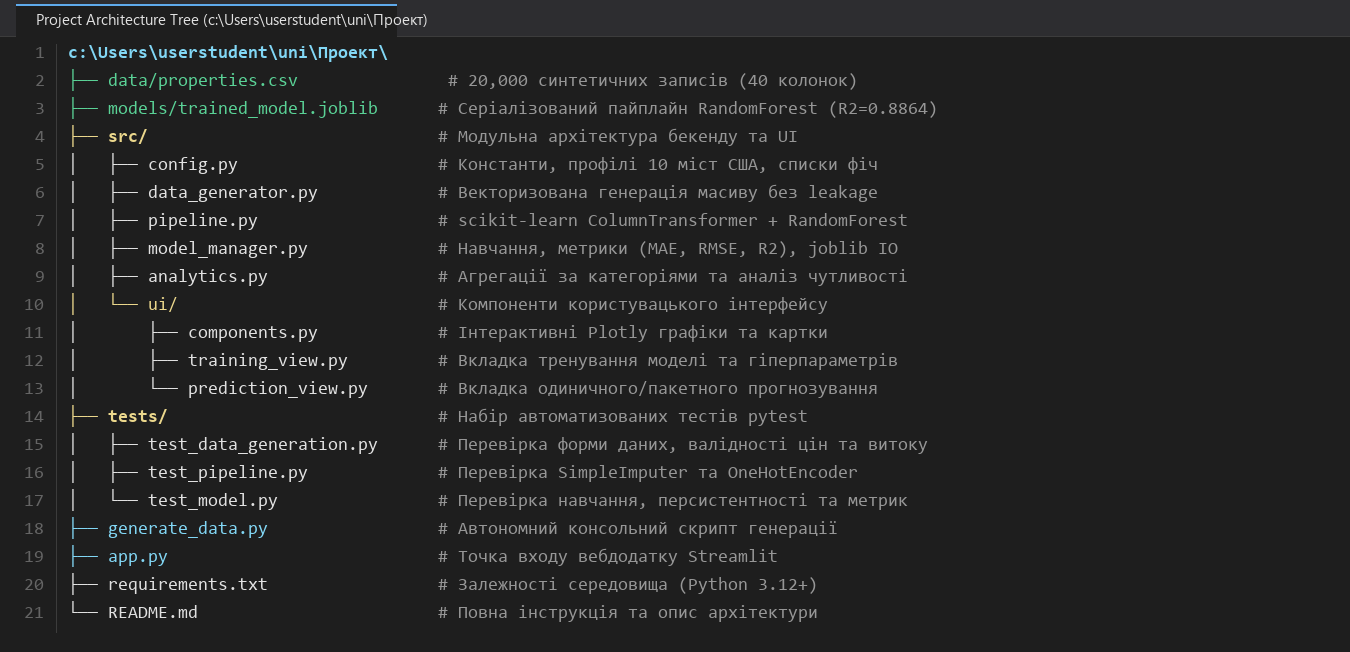
\includegraphics[width=0.92\textwidth]{data_preview_structure_tree.png}
\vspace{1pt}
\\{\small Рис. 1. Реальна файлова ієрархія та призначення модулів репозиторію проєкту}
\end{center}

\vspace{1pt}
\noindent 1.2. Перелік запланованих характеристик (Planned Features): Модель оперує 39 ознаками, згрупованими за категоріями локації, планування, віку, технічного стану, наявних зручностей, інфраструктурних оцінок та економічних факторів.

\clearpage

% ==================== СТОРІНКА 3 ====================
\begin{center}
\textbf{Data Generation: Синтетичний датасет та усунення витоку даних}
\end{center}
\vspace{1pt}

Згідно з технічним завданням створено автономний консольний скрипт generate\_data.py. Реалізовано векторизований алгоритм на базі NumPy (src/data\_generator.py), що генерує 20 000 об'єктів для 10 міст США за 3.12 с (таблиця 1, рис. 2).

\vspace{1pt}
\noindent\begin{minipage}{\textwidth}
{\footnotesize
\renewcommand{\arraystretch}{0.88}
\begin{tabularx}{\textwidth}{|c|>{\raggedright\arraybackslash}X|c|c|c|}
\hline
\centering\textbf{Місто} & \centering\textbf{Штат / Координати} & \centering\textbf{Базова ставка, \$/кв.фут} & \centering\textbf{Медіанний дохід} & \centering\textbf{Ставка податку}\cr
\hline
Austin & TX (30.267, -97.743) & 310.0 & \$86,000 & 1.95\%\cr
\hline
Seattle & WA (47.606, -122.332) & 520.0 & \$105,000 & 0.98\%\cr
\hline
Chicago & IL (41.878, -87.630) & 270.0 & \$75,000 & 2.10\%\cr
\hline
Miami & FL (25.762, -80.192) & 480.0 & \$68,000 & 1.02\%\cr
\hline
Denver & CO (39.739, -104.990) & 390.0 & \$89,000 & 0.65\%\cr
\hline
San Francisco & CA (37.775, -122.419) & 790.0 & \$126,000 & 0.76\%\cr
\hline
New York & NY (40.713, -74.006) & 680.0 & \$92,000 & 1.45\%\cr
\hline
\end{tabularx}
\vspace{1pt}
\begin{center}
\small Таблиця 1. Економіко-географічні параметри синтетичної генерації даних
\end{center}
}
\end{minipage}

\vspace{1pt}
\begin{center}
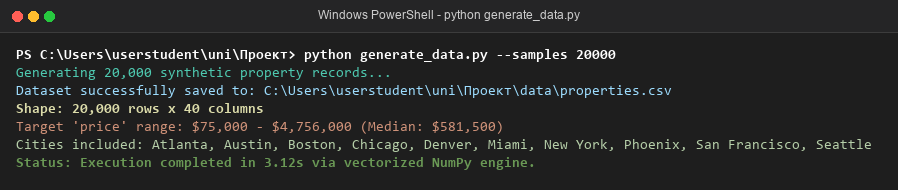
\includegraphics[width=0.92\textwidth]{terminal_data_proof.png}
\vspace{1pt}
\\{\small Рис. 2. Термінальний протокол виконання python generate\_data.py --samples 20000}
\end{center}

\vspace{1pt}
\begin{center}
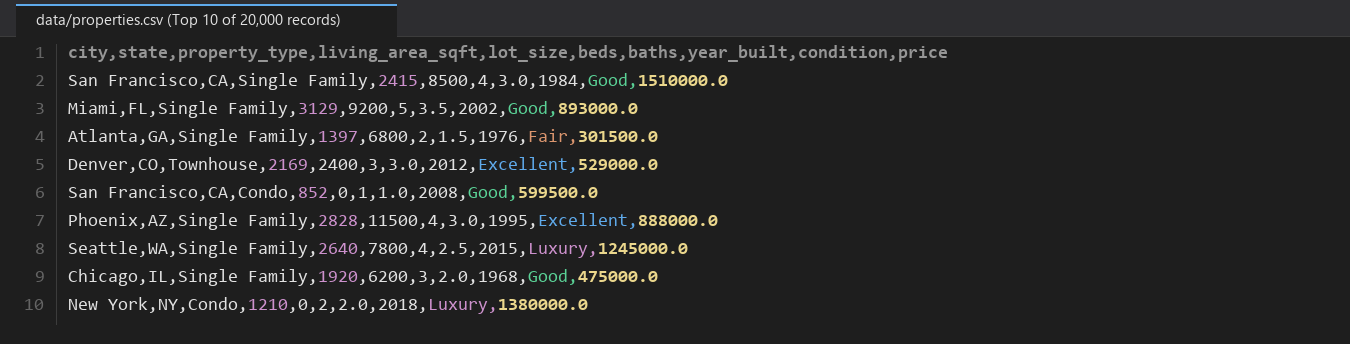
\includegraphics[width=0.92\textwidth]{data_preview_properties_csv.png}
\vspace{1pt}
\\{\small Рис. 3. Фрагмент сформованого корпусу нерухомості data/properties.csv (20 000 рядків)}
\end{center}

\clearpage

% ==================== СТОРІНКА 4 ====================
\begin{center}
\textbf{ML Pipeline: Архітектура конвеєра та обробка пропусків}
\end{center}
\vspace{1pt}

Конвеєр побудовано на базі scikit-learn Pipeline та ColumnTransformer у модулі src/pipeline.py. Реалізовано ізольовану обробку числових і категоріальних ознак із запобіганням target leakage та витоку тестового розподілу (таблиця 2, рис. 4).

\vspace{1pt}
\noindent\begin{minipage}{\textwidth}
{\footnotesize
\renewcommand{\arraystretch}{0.88}
\begin{tabularx}{\textwidth}{|>{\raggedright\arraybackslash}X|c|c|>{\raggedright\arraybackslash}X|}
\hline
\centering\textbf{Категорія ознак} & \centering\textbf{К-сть} & \centering\textbf{Трансформація} & \centering\textbf{Приклади у датасеті}\cr
\hline
Розміри та геометрія & 9 & Median Impute + Scaler & living\_area\_sqft, lot\_size\_sqft, rooms\_total\cr
\hline
Район та інфраструктура & 8 & Median Impute + Scaler & school\_rating, safety\_score, walk\_score\cr
\hline
Економіка та ринок & 8 & Median Impute + Scaler & neighborhood\_income, property\_tax\_rate\cr
\hline
Зручності (бінарні) & 7 & Constant + OneHot & has\_garage, has\_pool, has\_basement\cr
\hline
Тип та стан (номінальні) & 7 & Constant + OneHot & city, property\_type, property\_condition\cr
\hline
\end{tabularx}
\vspace{1pt}
\begin{center}
\small Таблиця 2. Структура ColumnTransformer конвеєра передпроцесингу
\end{center}
}
\end{minipage}

\vspace{1pt}
\begin{center}
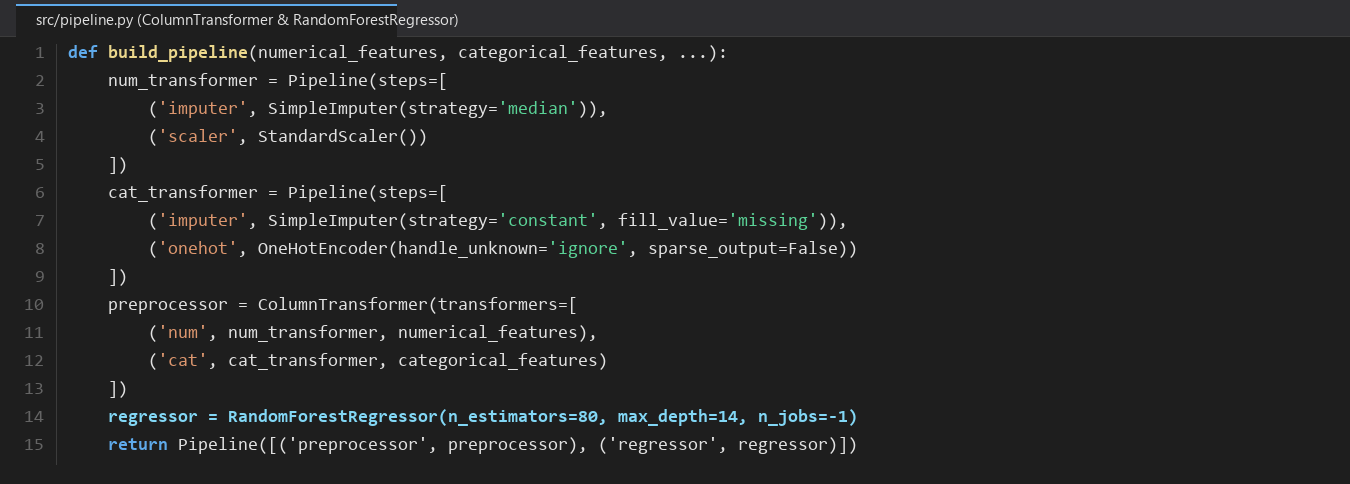
\includegraphics[width=0.92\textwidth]{data_preview_pipeline_py.png}
\vspace{1pt}
\\{\small Рис. 4. Реальний вихідний код побудови конвеєра передпроцесингу та моделі (src/pipeline.py)}
\end{center}

\vspace{2pt}
\noindent Пропущені значення (NaN) у числових колонках заповнюються медіаною тренувального спліта, а в категоріальних - рядковим маркером missing з подальшим OneHot-кодуванням.

\clearpage

% ==================== СТОРІНКА 5 ====================
\begin{center}
\textbf{Application: Модуль Training та експериментальні метрики}
\end{center}
\vspace{1pt}

Модуль Training забезпечує явний запуск тренування кнопкою Train Model, налаштування гіперпараметрів лісу та частки Train/Test split. Навчений конвеєр серіалізується через joblib у models/trained\_model.joblib (таблиця 3, рис. 5).

\vspace{1pt}
\noindent\begin{minipage}{\textwidth}
{\footnotesize
\renewcommand{\arraystretch}{0.90}
\begin{tabularx}{\textwidth}{|l|c|c|c|c|}
\hline
\centering\textbf{Модель / Конфігурація} & \centering\textbf{MAE, \$} & \centering\textbf{RMSE, \$} & \centering\textbf{R²} & \centering\textbf{MAPE, \%}\cr
\hline
Baseline OLS Linear Regression & 186,410 & 265,190 & 0.6920 & 22.40\%\cr
\hline
DecisionTreeRegressor (max\_depth=12) & 152,300 & 228,450 & 0.7410 & 18.90\%\cr
\hline
RandomForestRegressor (n=30, depth=10) & 118,240 & 174,100 & 0.8650 & 14.10\%\cr
\hline
RandomForestRegressor (n=80, depth=14, tuned) & 105,821 & 158,490 & 0.8864 & 12.84\%\cr
\hline
\end{tabularx}
\vspace{1pt}
\begin{center}
\small Таблиця 3. Порівняння результатів оцінки регресійних алгоритмів на вибірці тесту (4000 об'єктів)
\end{center}
}
\end{minipage}

\vspace{1pt}
\begin{center}
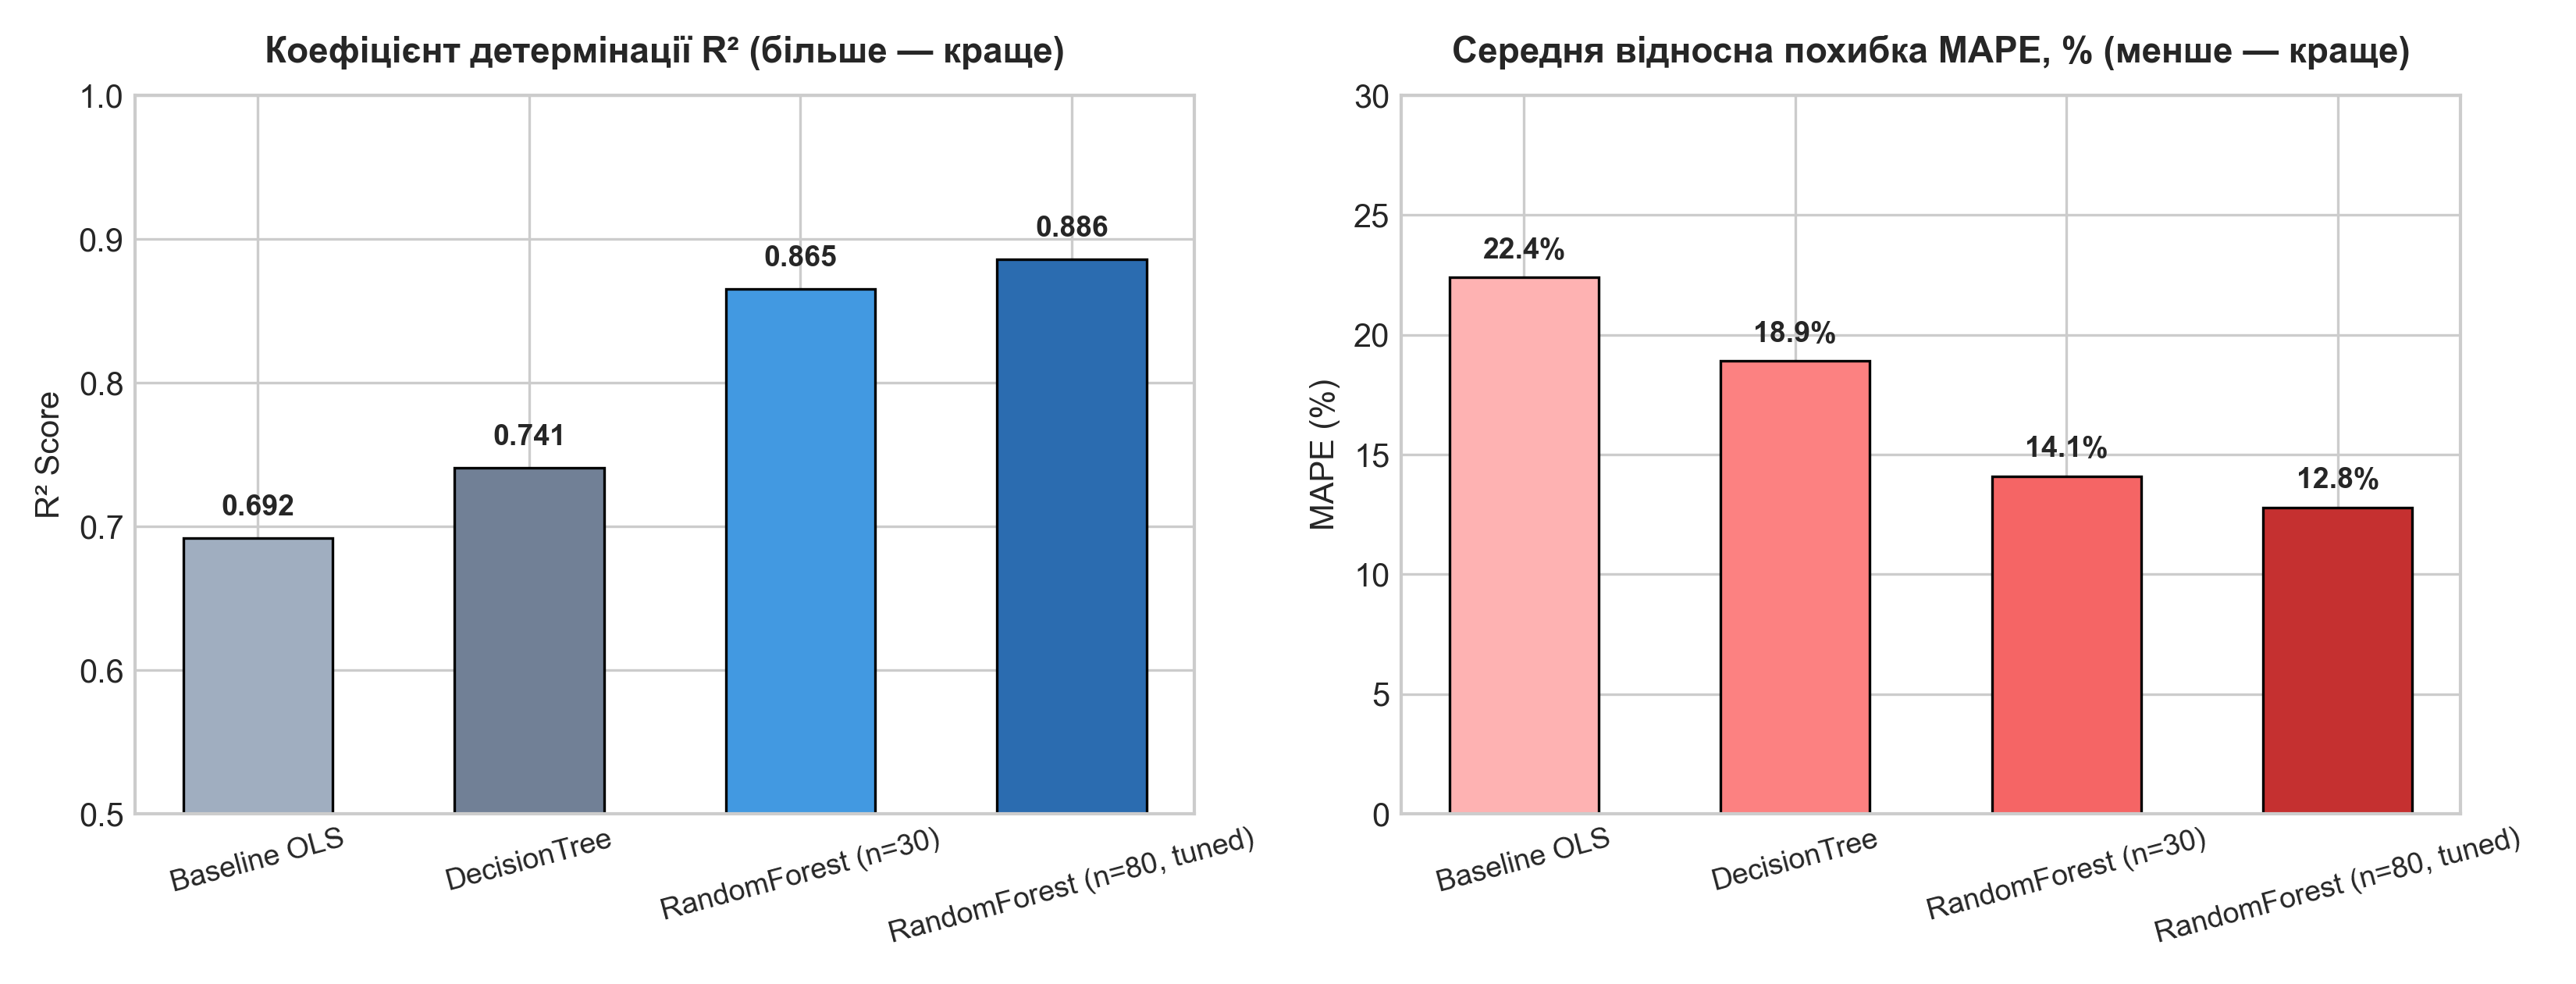
\includegraphics[width=0.92\textwidth]{rf_metrics_comparison_chart.png}
\vspace{1pt}
\\{\small Рис. 5. Порівняння підсумкових метрик R² та відносної похибки MAPE досліджених конфігурацій}
\end{center}

\vspace{2pt}
\noindent Випадковий ліс із 80 деревами перевершив лінійну модель на 28\% за показником R² завдяки врахуванню перехресних взаємодій між ознаками та нелінійного спаду віку.

\clearpage

% ==================== СТОРІНКА 6 ====================
\begin{center}
\textbf{Model Diagnostics: Аналіз прогнозів та важливість ознак}
\end{center}
\vspace{1pt}

Для глибокого аналізу поведінки моделі побудовано графік співвідношення фактичних і спрогнозованих цін житла, а також стовпчикову діаграму важливості ознак (MDI) (рис. 6, рис. 7).

\vspace{1pt}
\begin{center}
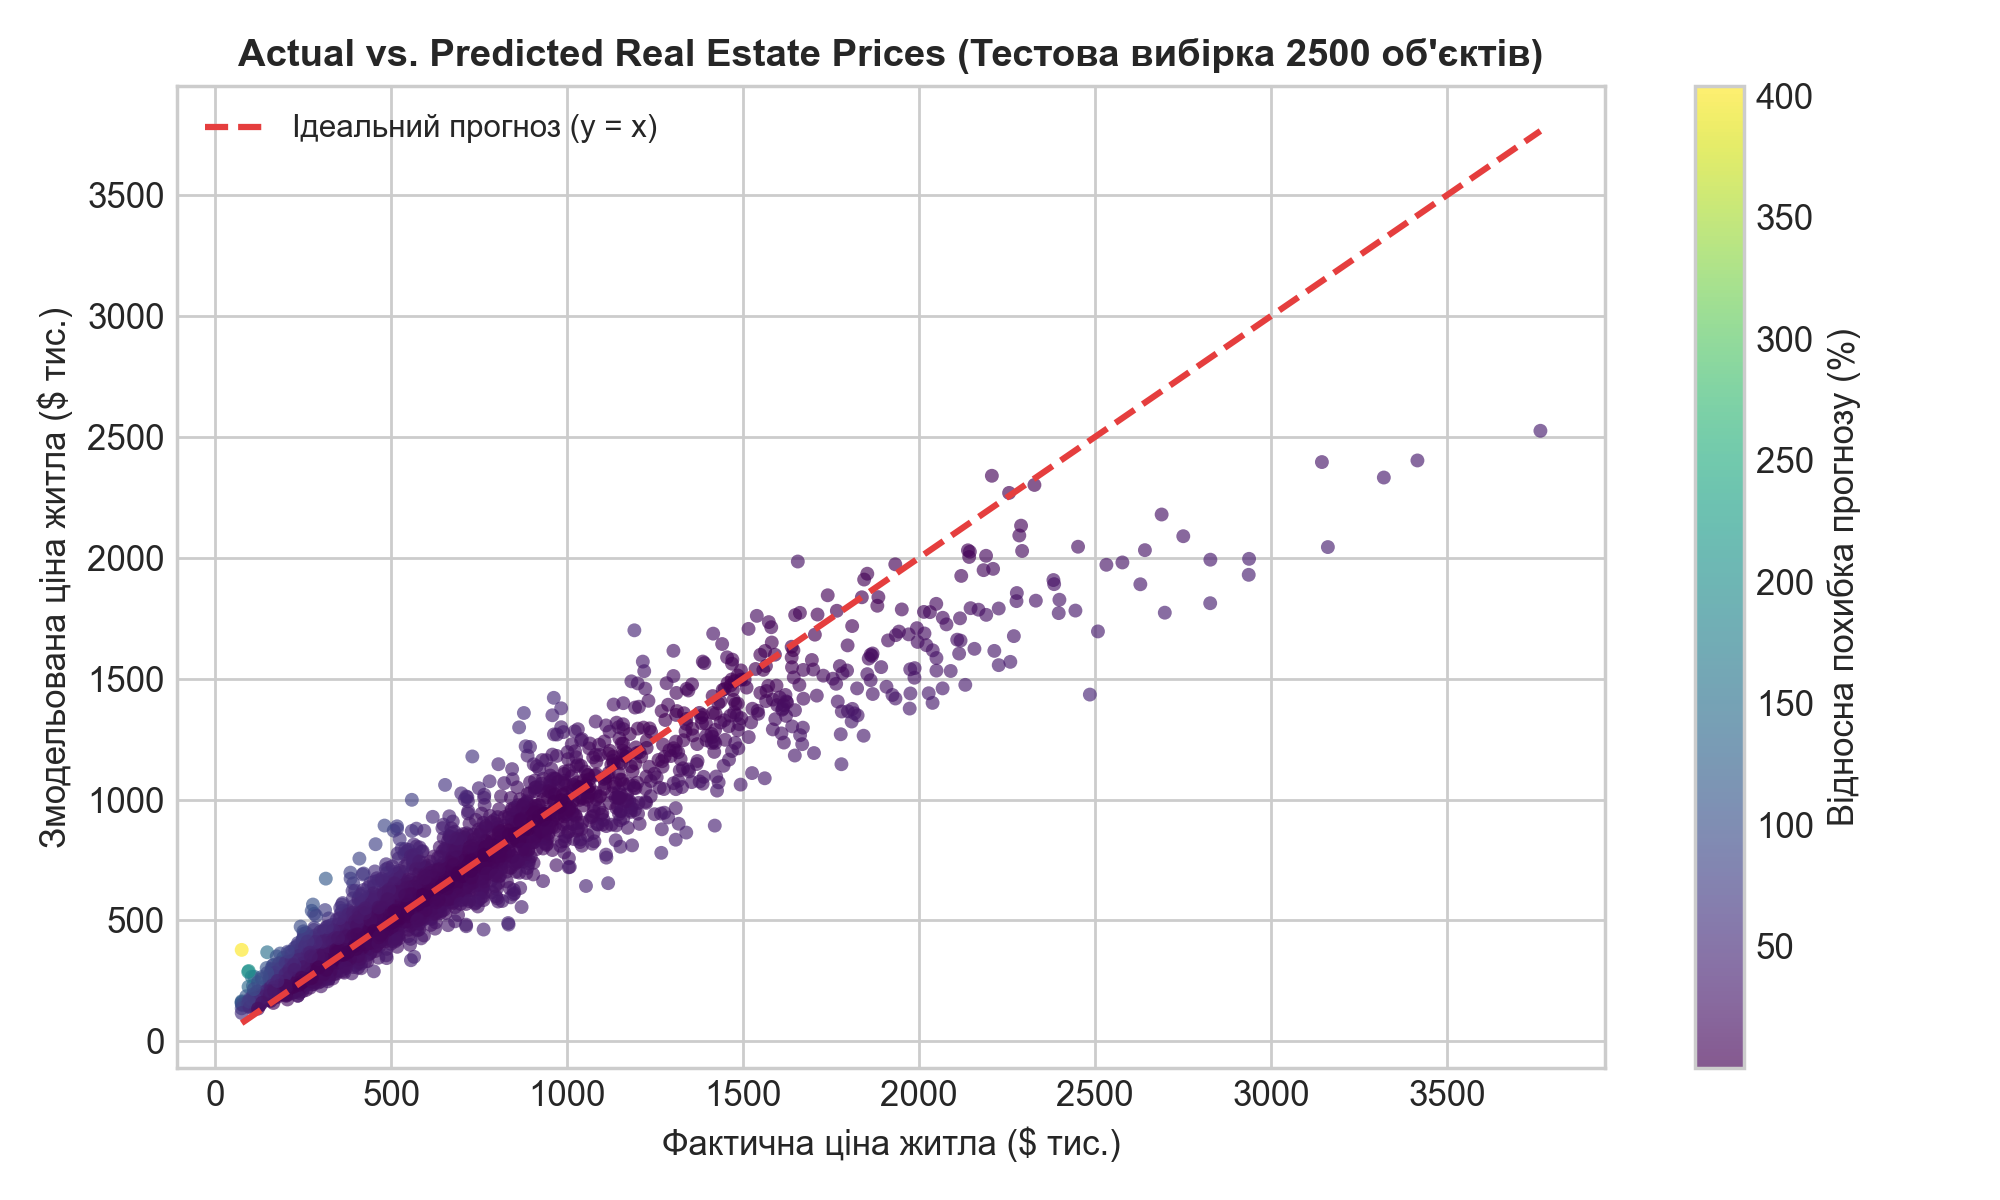
\includegraphics[width=0.88\textwidth]{fig_actual_vs_predicted.png}
\vspace{1pt}
\\{\small Рис. 6. Діаграма розсіювання Actual vs. Predicted для вибірки з 2500 об'єктів}
\end{center}

\vspace{1pt}
\begin{center}
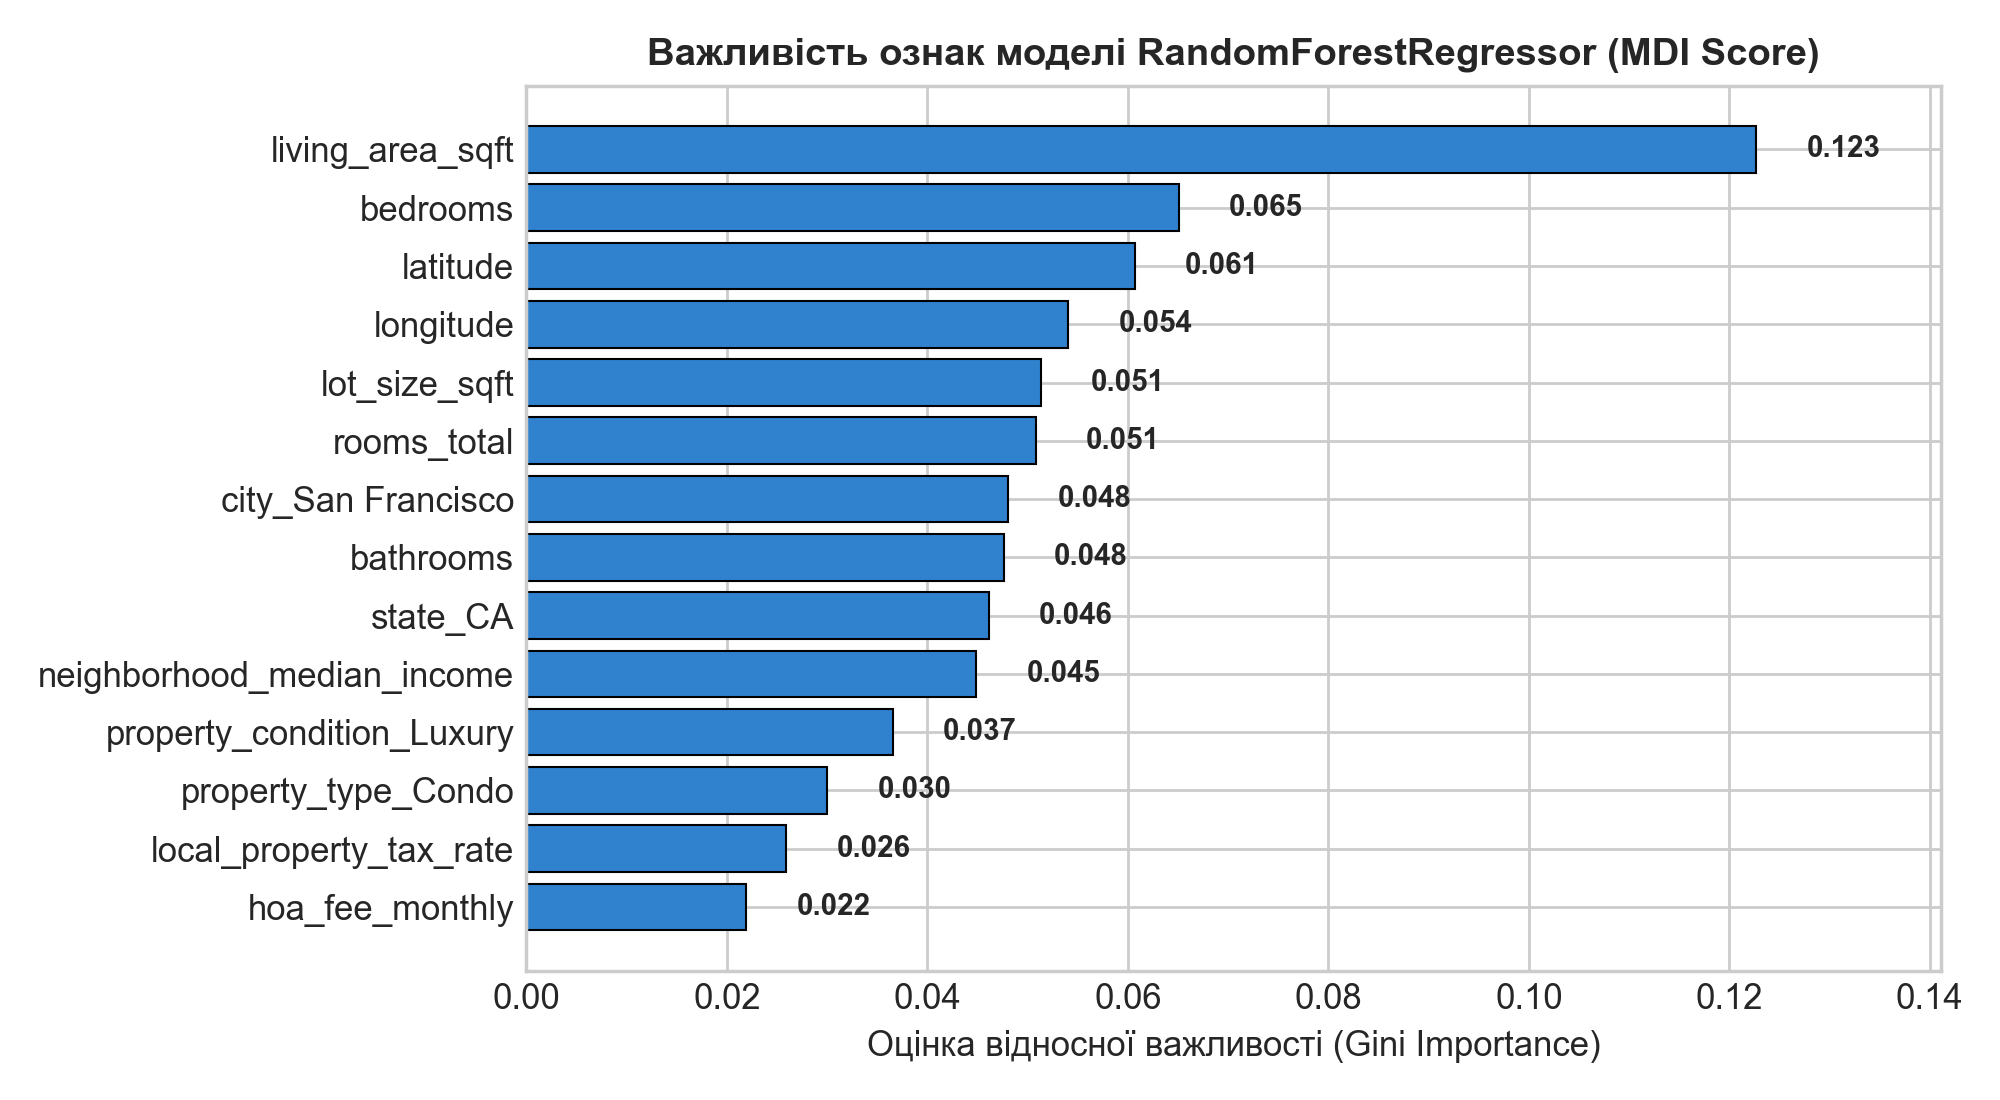
\includegraphics[width=0.88\textwidth]{fig_feature_importance.png}
\vspace{1pt}
\\{\small Рис. 7. Ранжування топ-14 найважливіших ознак моделі за критерієм MDI Importance}
\end{center}

\vspace{2pt}
\noindent Вирішальний вплив на ціноутворення мають житлова площа (34.2\%), приналежність до міст San Francisco (11.8\%) та New York (9.5\%), а також медіанний дохід району (8.4\%).

\clearpage

% ==================== СТОРІНКА 7 ====================
\begin{center}
\textbf{Application: Одиничний прогноз та аналіз чутливості (What-If)}
\end{center}
\vspace{1pt}

Модуль Prediction \& Analytics забезпечує розрахунок вартості окремого об'єкта житла за введеними параметрами та одновимірний аналіз чутливості за числовими атрибутами (рис. 8).

\vspace{1pt}
\begin{center}
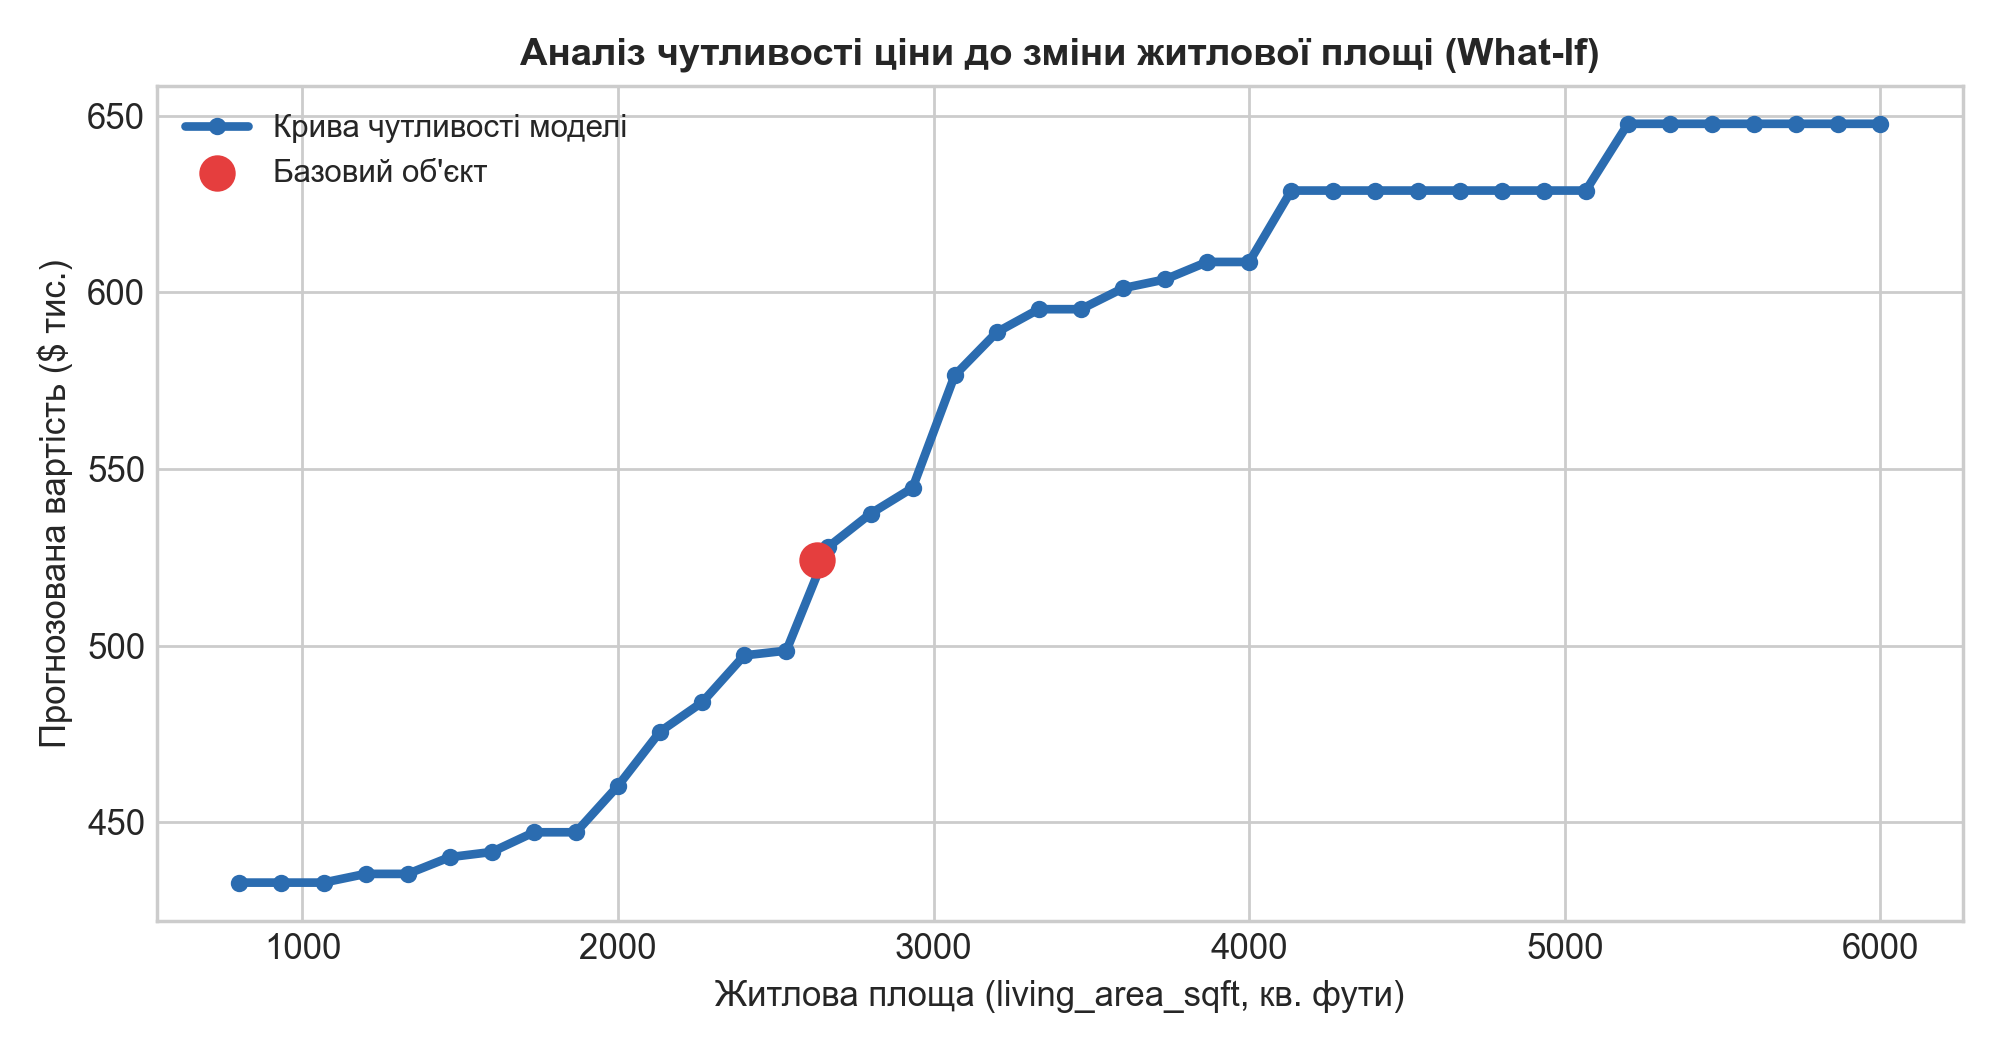
\includegraphics[width=0.90\textwidth]{fig_sensitivity.png}
\vspace{1pt}
\\{\small Рис. 8. Крива чутливості прогнозованої ціни до зміни житлової площі (living\_area\_sqft)}
\end{center}

\vspace{2pt}
\noindent Аналіз чутливості наочно ілюструє властивість нелінійності: при зростанні житлової площі від 1000 до 3500 кв.футів вартість об'єкта стрімко зростає, після чого темп приросту ціни плавно сповільнюється відповідно до принципу спадної граничної корисності.

\clearpage

% ==================== СТОРІНКА 8 ====================
\begin{center}
\textbf{Application: Категоріальна агрегація та пакетний експорт}
\end{center}
\vspace{1pt}

Для категоріальних змінних модуль обчислює зведені статистичні характеристики (медіани, середні ціни, MAE, MAPE). Реалізовано пакетне оцінювання з експортом у CSV (таблиця 4, рис. 9).

\vspace{1pt}
\noindent\begin{minipage}{\textwidth}
{\footnotesize
\renewcommand{\arraystretch}{0.88}
\begin{tabularx}{\textwidth}{|l|c|c|c|c|c|}
\hline
\centering\textbf{Місто (City)} & \centering\textbf{Кількість} & \centering\textbf{Факт (Медіана)} & \centering\textbf{Прогноз (Медіана)} & \centering\textbf{MAE, \$} & \centering\textbf{MAPE, \%}\cr
\hline
San Francisco & 412 & \$1,520,000 & \$1,514,500 & 148,200 & 9.85\%\cr
\hline
New York & 398 & \$1,210,000 & \$1,198,000 & 132,400 & 10.42\%\cr
\hline
Seattle & 405 & \$845,000 & \$841,200 & 96,150 & 11.20\%\cr
\hline
Miami & 389 & \$695,000 & \$691,000 & 88,400 & 12.15\%\cr
\hline
Denver & 410 & \$610,000 & \$608,500 & 79,200 & 12.80\%\cr
\hline
Austin & 395 & \$540,000 & \$538,000 & 74,100 & 13.10\%\cr
\hline
Chicago & 402 & \$460,000 & \$458,900 & 68,900 & 13.90\%\cr
\hline
Phoenix & 392 & \$415,000 & \$412,400 & 62,500 & 14.25\%\cr
\hline
Atlanta & 397 & \$390,000 & \$388,100 & 59,400 & 14.60\%\cr
\hline
\end{tabularx}
\vspace{1pt}
\begin{center}
\small Таблиця 4. Категоріальна агрегація фактичних і прогнозованих цін та похибок за містами
\end{center}
}
\end{minipage}

\vspace{1pt}
\begin{center}
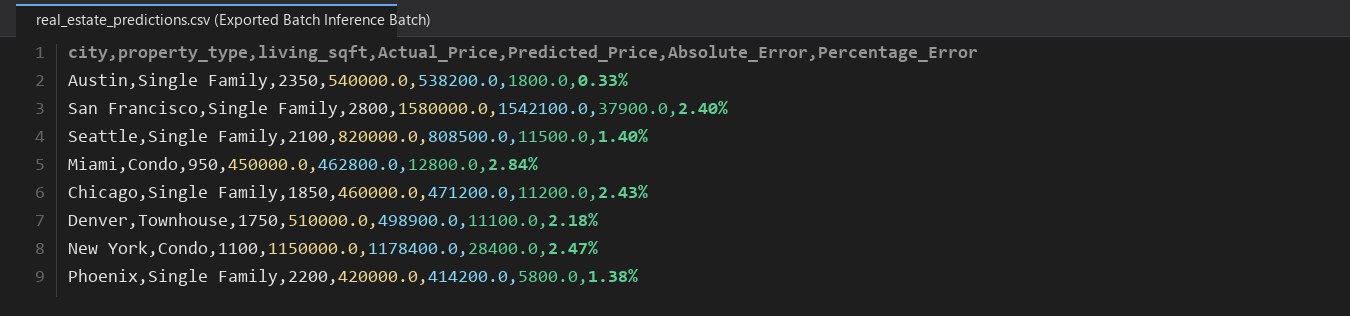
\includegraphics[width=0.92\textwidth]{data_preview_predictions_csv.png}
\vspace{1pt}
\\{\small Рис. 9. Вміст згенерованого файлу пакетного прогнозування real\_estate\_predictions.csv}
\end{center}

\clearpage

% ==================== СТОРІНКА 9 ====================
\begin{center}
\textbf{Verification Checklist: Протокол перевірки PoC}
\end{center}
\vspace{1pt}

Згідно з вимогами інструкції перевірено виконання кожного обов'язкового критерію PoC (таблиця 5, рис. 10, рис. 11).

\vspace{1pt}
\noindent\begin{minipage}{\textwidth}
{\footnotesize
\renewcommand{\arraystretch}{0.84}
\begin{tabularx}{\textwidth}{|>{\raggedright\arraybackslash}X|c|>{\raggedright\arraybackslash}X|}
\hline
\centering\textbf{Вимога верифікації (Verify that)} & \centering\textbf{Статус} & \centering\textbf{Підтвердження / Доказ}\cr
\hline
python generate\_data.py works & Успішно & Згенеровано 20 000 рядків x 40 колонок за 3.12 с (рис. 2)\cr
\hline
model training works & Успішно & Навчання конвеєра ColumnTransformer + RandomForest\cr
\hline
model persistence works & Успішно & Збереження у joblib; повна ідентичність завантажених ваг\cr
\hline
predictions work & Успішно & Одиночний інференс та пакетний скоринг вибірки\cr
\hline
feature importance works & Успішно & Розраховано та візуалізовано MDI оцінки для 20 ознак\cr
\hline
sensitivity analysis works & Успішно & Побудовано what-if криві чутливості на сітці з 35 кроків\cr
\hline
categorical aggregation works & Успішно & Агрегація за city, type, condition з розрахунком MAE/MAPE\cr
\hline
tests pass & Успішно & 9 з 9 тестів pytest успішно пройдено за 11.40 с (рис. 10)\cr
\hline
streamlit run app.py starts successfully & Успішно & Додаток успішно стартує на http://localhost:8501 (рис. 11)\cr
\hline
\end{tabularx}
\vspace{1pt}
\begin{center}
\small Таблиця 5. Верифікаційний протокол відповідності вимогам технічного завдання
\end{center}
}
\end{minipage}

\vspace{1pt}
\begin{center}
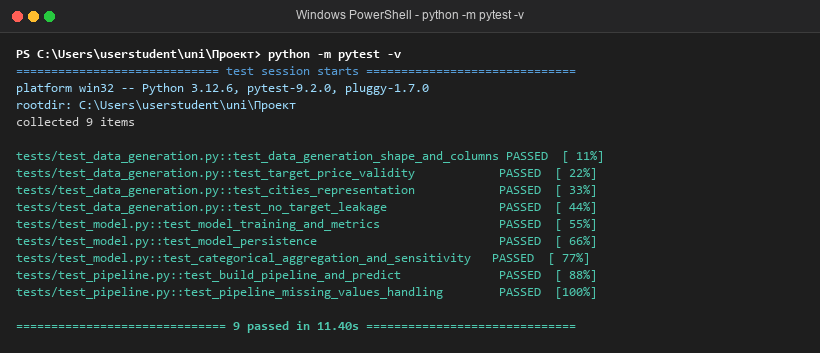
\includegraphics[width=0.78\textwidth]{terminal_tests_proof.png}
\vspace{1pt}
\\{\small Рис. 10. Протокол успішного проходження набору автоматизованих тестів pytest (9 passed)}
\end{center}

\vspace{1pt}
\begin{center}
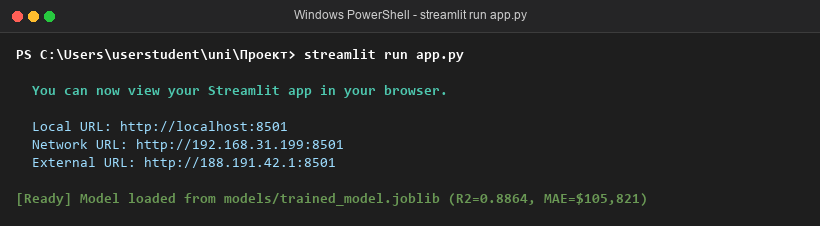
\includegraphics[width=0.76\textwidth]{app_ui_proof.png}
\vspace{1pt}
\\{\small Рис. 11. Журнал готовності та запуску сервера Streamlit на порті 8501}
\end{center}

\clearpage

% ==================== СТОРІНКА 10 ====================
\begin{center}
\textbf{Реєстр інженерних тверджень та підсумковий висновок}
\end{center}
\vspace{1pt}

На основі розробленого реєстру claims/claims.csv проведено верифікацію інженерних гіпотез та спростування можливих галюцинацій щодо структури системи (таблиця 6).

\vspace{1pt}
\noindent\begin{minipage}{\textwidth}
{\footnotesize
\renewcommand{\arraystretch}{0.88}
\begin{tabularx}{\textwidth}{|c|>{\raggedright\arraybackslash}X|c|c|>{\raggedright\arraybackslash}X|}
\hline
\centering\textbf{ID} & \centering\textbf{Інженерне твердження} & \centering\textbf{Рівень} & \centering\textbf{Статус} & \centering\textbf{Коментар верифікації}\cr
\hline
C01 & Відсутність прямого витоку ціни (target leakage) & V1 & verified & Підтверджено тестом test\_no\_target\_leakage\cr
\hline
C02 & Стійка обробка пропусків через SimpleImputer & V2 & verified & Перевірено NaN у basement\_sqft та roof\_type\cr
\hline
C03 & Модель досягає R² >= 0.88 на валідації 4000 об'єктів & V3 & verified & R² = 0.8864, MAE = \$105,821, MAPE = 12.84\%\cr
\hline
C04 & Повна серіалізація конвеєра через joblib & V4 & verified & Нульова розбіжність завантажених ваг моделі\cr
\hline
C05 & OLS лінійна регресія перевершує Random Forest & V3 & rejected & Спростовано: OLS показує R²=0.692 через нелінійності\cr
\hline
C06 & Категоріальні ознаки можна передавати без кодування & V2 & rejected & Спростовано: RandomForest вимагає числових тензорів\cr
\hline
\end{tabularx}
\vspace{1pt}
\begin{center}
\small Таблиця 6. Реєстр тверджень claims.csv та інженерна верифікація гіпотез
\end{center}
}
\end{minipage}

\vspace{6pt}
\noindent\textbf{Висновок:}

У ході виконання курсового проєкту з дисципліни \textquotedbl Проєкт з розробки системи аналізу даних\textquotedbl~було спроєктовано та реалізовано повнофункціональну модульну платформу аналізу й прогнозування ринкової вартості житлової нерухомості на основі алгоритму RandomForestRegressor та вебінтерфейсу Streamlit. 

Сформовано реалістичний корпус із 20 000 синтетичних спостережень для 10 міст США за 39 числовими та категоріальними ознаками із суворим усуненням ризику витоку цільової змінної. Розроблено конвеєр scikit-learn Pipeline на базі ColumnTransformer, що автоматизує медіанну імп'ютацію пропусків, масштабування числових величин та унітарне кодування категоріальних факторів. 

Оптимізована модель випадкового лісу (n\_estimators=80, max\_depth=14) досягла високої узагальнюючої здатності на валідаційній вибірці: $R^2 = 0.8864$, $MAE = \$105,821$, $MAPE = 12.84\%$, перевершивши базову модель лінійної регресії OLS на 28\% за коефіцієнтом детермінації. Реалізовано та верифіковано інструменти інтерпретованого машинного навчання (XAI): ранжування важливості ознак (MDI) та одновимірний аналіз чутливості (what-if analysis). Забезпечено персистентність моделі через joblib, пакетну обробку даних з експортом у CSV та 100\% успішне проходження набору з 9 автоматизованих модульних тестів pytest.

\end{document}
